\documentclass[conference]{IEEEtran}
\IEEEoverridecommandlockouts
\usepackage{cite}
\usepackage{amsmath,amssymb,amsfonts}
\usepackage{graphicx}
\usepackage{textcomp}
\usepackage{xcolor}
\newcommand{\todo}[1]{\textcolor{red}{[TBD: #1]}}

\begin{document}

\title{An Automated Scan-to-Simulation Pipeline for Indoor Digital Twin
Construction Using BLK360 and NVIDIA Isaac Sim}

% RAAICON 2026 double-blind: 초기 제출본에는 저자/소속/이메일/사사 금지.
% 저자 정보는 CMT에만 입력. camera-ready 때 아래 블록을 실제 저자로 교체.
\author{\IEEEauthorblockN{Anonymous Authors}
\IEEEauthorblockA{Paper ID: XXXX (double-blind submission)}
}

\maketitle

\begin{abstract}
Constructing a simulation environment that faithfully reproduces a real
indoor workspace is a major bottleneck when deploying digital twins for
mobile robots: scenes are typically modeled by hand, which is slow,
subjective, and quickly outdated. This paper presents an automated
scan-to-simulation pipeline that converts a single terrestrial laser
scan of an industrial indoor space into a physics-enabled, photorealistic
NVIDIA Isaac Sim environment, and couples it with a real mobile
manipulator to form a live bidirectional digital twin. A Leica BLK360
point cloud of 68.5 million points is automatically processed into
(i) a 2D occupancy grid via floor-plane estimation and height-band
rasterization, (ii) a collidable wall geometry layer for physics
simulation, and (iii) a dense colored point-cloud layer for visual
fidelity. A swerve-drive mobile manipulator modeled from 2D CAD drawings
is embedded in the scene, and a ROS 2 DDS bridge mirrors the real robot
pose at 30 Hz while navigation goals selected inside the simulator are
dispatched to the on-board navigation stack. A one-shot anchor-based
calibration aligns the robot localization frame with the scan frame.
The full conversion completes in under 80 seconds on a desktop
workstation, and the resulting 3.7-million-point scene simulates at
5.6 times real time in physics-only mode and above 100 rendered frames
per second in the interactive viewport. On-site experiments with the
physical robot show that the reconstructed scene preserves metric scale
to within 2\% of tape-measured room dimensions, that end-to-end twin
positioning agrees with tape-measured checkpoint distances to 5.5 cm
mean absolute error, and that navigation goals issued inside the
simulator drive the real robot to the commanded locations.
\end{abstract}

\begin{IEEEkeywords}
digital twin, terrestrial laser scanning, scan-to-simulation,
mobile robot, NVIDIA Isaac Sim, ROS 2
\end{IEEEkeywords}

\section{Introduction}
Digital twins---virtual replicas of physical assets that stay
synchronized with their real counterparts---are increasingly adopted in
manufacturing and logistics for commissioning, monitoring, and operator
training of mobile robot fleets \cite{tao2019}. A prerequisite for any
robot-level digital twin is a simulation environment that reproduces the
geometry of the real workspace with sufficient fidelity: collision
surfaces must be metrically accurate for navigation and motion planning,
and the visual appearance must be recognizable for human operators.

In practice, such environments are still largely modeled by hand. CAD
floor plans, when available, rarely reflect the as-is state of a
facility, and manual 3D modeling of clutter, racks, and equipment can
take days per room while introducing subjective simplifications.
Terrestrial laser scanners (TLS) such as the Leica BLK360 capture
dense, millimeter-accurate colored point clouds of indoor spaces in
minutes \cite{blk360}, but a raw point cloud is not a simulation
environment: it has no collision representation, no gravity-aligned
reference frame, and no interface to a robot simulator.

This paper addresses the gap with an automated scan-to-simulation
pipeline targeting NVIDIA Isaac Sim \cite{isaacsim}, coupled with a
live-twin runtime for a real swerve-drive autonomous mobile manipulator
robot (AMMR). Our contributions are:
\begin{itemize}
\item An automated conversion from a merged E57 TLS export to a
physics-ready Isaac Sim USD stage, comprising floor-plane estimation by
RANSAC \cite{ransac}, height-band occupancy-grid rasterization,
synthesis of collidable-but-invisible wall geometry, and a
voxel-downsampled colored point-cloud layer for visual fidelity.
\item A live bidirectional digital twin: the real robot pose is
mirrored in simulation at 30 Hz over a ROS 2 \cite{ros2} DDS bridge,
and navigation goals picked inside the simulator are dispatched to the
robot's on-board Nav2 \cite{nav2} stack. A one-shot anchor-based
calibration solves the SE(2) offset between the robot localization
frame and the scan frame.
\item A quantitative evaluation of the pipeline covering conversion
time (under 80 s end to end), scene complexity, simulation throughput
(5.6$\times$ real time physics-only; near real time with rendering),
and geometric fidelity of the twin against tape-measured ground-truth
distances.
\end{itemize}

Unlike approaches that reconstruct watertight meshes from scans, we
deliberately keep two decoupled layers---a coarse collision layer
derived from the occupancy grid and a dense point layer for
appearance---which keeps conversion fast, robust to scan noise, and
directly navigable by a mobile base.

\section{Related Work}
\subsection{As-built capture and scan-to-model conversion}
Automatic reconstruction of as-built environment models from point
clouds has been studied extensively in the construction domain
(scan-to-BIM) \cite{scan2bim}. These methods target semantically rich
building models and typically require minutes to hours per scene;
their output (IFC/BIM) is not directly consumable by robot simulators.
Game-engine-based reconstruction pipelines produce visually convincing
meshes but seldom guarantee the metric consistency required for
navigation. Our pipeline trades semantic richness for speed and
robustness, producing a physics-consistent simulation stage in tens of
seconds.

\subsection{Robot simulators and digital twins}
Gazebo \cite{gazebo} has long been the default simulator in the ROS
ecosystem; NVIDIA Isaac Sim adds GPU-accelerated PhysX simulation,
OpenUSD scene composition, and photorealistic rendering, and has been
adopted for robot learning \cite{orbit} and sim-to-real research
\cite{sim2real}. Existing Isaac Sim workflows, however, assume the
environment is authored beforehand. On the twin side, most reported
robot digital twins mirror robot state into a manually built scene.
The combination presented here---an automatically scan-built Isaac Sim
scene coupled bidirectionally to a real mobile manipulator---has, to
the best of our knowledge, not been quantitatively characterized before.

\section{Scan-to-Simulation Pipeline}
Fig.~\ref{figpipe} shows the system. The offline stage (top row)
converts a TLS scan into an Isaac Sim USD stage; the online stage
(bottom row) couples the stage to the real robot.

\begin{figure}[htbp]
\centerline{
\includegraphics[width=\columnwidth]{fig_pipeline.png}}
\caption{System overview. Offline (top): the merged BLK360 E57 export is
converted into an occupancy grid, a collidable wall layer, and a dense
colored point layer composing the Isaac Sim stage. Online (bottom): a
ROS 2 DDS bridge mirrors the robot pose at 30 Hz and returns navigation
goals selected in the simulator.}
\label{figpipe}
\end{figure}

\subsection{Scan acquisition and preprocessing}
The test space, an industrial test room of approximately
$13\times9$ m, was captured with a Leica BLK360 from multiple
viewpoints; scan placement followed a visibility-coverage plan, and the
registered stations were exported as a single E57 file (68.5 M points,
1.3 GB). The pipeline first estimates the dominant floor plane with
RANSAC on a voxel-thinned subset, yielding the gravity-aligned
reference frame and the floor height $z_0$; all subsequent layers are
expressed relative to this frame, so no manual leveling or origin
selection is required.

\subsection{Occupancy grid and collision layer}
Points within a height band $[z_0{+}0.10, z_0{+}1.80]$ m---the band
relevant for a mobile base---are rasterized into a 2D occupancy grid at
0.05 m resolution ($654\times474$ cells for the full scan extent).
Morphological cleanup removes speckle from reflections and small
blobs below 0.02 m$^2$. The occupied cells are then greedily merged
into axis-aligned boxes and emitted as USD cubes of 2.5 m height with
PhysX collision enabled. Crucially, the collision boxes are marked
\emph{invisible}: they provide physics without occluding the visual
point layer. The same occupancy grid is exported in ROS map format
(PGM/YAML) so that the simulated and real navigation stacks can share
one map.

\subsection{Visual point-cloud layer}
For appearance, the full-resolution colored cloud is voxel-downsampled
to 0.015 m (3.6 M points, ceiling included) and embedded as USD
\texttt{Points} prims with per-point color and a rendered point width
of 0.013 m, chosen at approximately 0.8 times the voxel size so points
visually fuse into surfaces at navigation-relevant viewing distances.
The two-layer design keeps the stage lightweight: collision queries
run against 1{,}430 boxes rather than millions of points, while the
operator sees the photographic appearance of the real room.

\subsection{Robot model and mobile-base control}
The AMMR is a swerve-drive mobile manipulator with two independently
steered wheel modules mounted diagonally at $\mathbf{p}_{1,2}=
(\pm0.364, \mp0.137)$ m and four passive casters. Its URDF (12 links,
11 joints) was authored from the manufacturer's 2D drawings. For
simulation-only operation the base is velocity-controlled through the
standard inverse kinematics: for a commanded body twist
$(v_x, v_y, \omega)$ each module $i$ tracks
\begin{equation}
\mathbf{v}_i = \begin{bmatrix} v_x - \omega\, p_{i,y} \\
v_y + \omega\, p_{i,x} \end{bmatrix},\quad
\delta_i = \operatorname{atan2}(v_{i,y}, v_{i,x}),\quad
\dot\varphi_i = \frac{\lVert \mathbf{v}_i \rVert}{r}
\label{eq:swerve}
\end{equation}
with wheel radius $r=0.075$ m. Steering angles are wrapped to
$[-90^\circ, 90^\circ]$ with wheel-speed reversal; a hysteresis of
0.12 rad on the reversal decision and a $\cos$ speed gate suppress the
flip-flopping that otherwise occurs when a module operates exactly at
the wrap boundary (e.g., during pure rotation).

\subsection{Live twin bridge and frame calibration}
During live operation the simulated robot is switched to kinematic
mode and mirrors the real pose. The robot publishes its localized pose
(TF $map\rightarrow base$, AMCL) as a 30 Hz odometry stream; the
simulator subscribes over a DDS bridge (Cyclone DDS \cite{cyclonedds},
dedicated domain, unicast peer configuration over Wi-Fi) and applies
the pose each physics step. In the reverse direction, dragging a goal
marker in the simulator publishes a goal pose that an on-robot relay
forwards to Nav2, closing the loop: the physical robot navigates to
targets picked in the twin.

The robot's SLAM map frame and the scan frame differ by an unknown
planar rigid transform. We calibrate it with a single anchor: the
robot is parked at a physically identifiable spot whose scan-frame
pose $(\mathbf{a}, \theta_a)$ is known---in our case the robot itself
was captured in the scan, so its scanned footprint provides the
anchor. On receipt of the first live pose $(\mathbf{r}, \theta_r)$ the
offset is closed-form:
\begin{equation}
\theta_{\mathrm{off}} = \theta_a - \theta_r, \qquad
\mathbf{t}_{\mathrm{off}} = \mathbf{a} - R(\theta_{\mathrm{off}})\,\mathbf{r}
\label{eq:anchor}
\end{equation}
and is reused for all subsequent poses and goals.

\section{Experimental Results}
All experiments ran on a desktop workstation (AMD Ryzen 9 9900X,
NVIDIA RTX PRO 4000 Blackwell 24 GB, Isaac Sim 5.1, ROS 2 Jazzy).

\subsection{Conversion time}
Table~\ref{tabtime} reports single-run wall-clock times for each
pipeline stage on the 68.5 M-point scan. The complete conversion from
raw E57 to a simulation-ready USD stage takes 78.5 s; the dominant
cost is writing the 3.7 M-point visual layer. A reduced-density
variant (485 k points) completes in 36.5 s. Authoring a comparable
environment by hand is a multi-day effort, and unlike manual modeling
the pipeline can be rerun after every facility change.

\begin{table}[htbp]
\caption{Scan-to-simulation conversion time (68.5 M-point E57)}
\begin{center}
\begin{tabular}{|l|r|}
\hline
\textbf{Stage} & \textbf{Time [s]} \\
\hline
Floor RANSAC, occupancy grid, ROS map export & 14.8 \\
Dense visual cloud extraction (voxel 0.015 m) & 16.8 \\
Visual layer USD export (3.7 M points) & 46.8 \\
Collision-layer synthesis (1{,}430 boxes) & 0.1 \\
\hline
\textbf{Total} & \textbf{78.5} \\
\hline
\end{tabular}
\label{tabtime}
\end{center}
\end{table}

\subsection{Scene complexity and simulation performance}
The generated stage contains 1{,}430 collision boxes
($\approx$17 k triangles) and 3{,}725{,}047 rendered points (166 MB
USD). With the AMMR articulation loaded (physics at 120 Hz),
headless physics-only simulation advances at 675 steps/s, a real-time
factor (RTF) of 5.64; with rendering enabled the simulator sustains
51 rendered frames per second (RTF 0.84). Rates were measured as the
simulation-clock publication rate over 30 s windows. In the interactive
GUI session used for the on-site experiments below, the viewport
sustained 104 frames per second (9.6 ms frame time) with the full point
layer in view.

\subsection{Simulation-only base control validation}
Before coupling to the real robot, the swerve base was validated in
simulation: straight-line, lateral (strafe), and in-place rotation
commands produce odometry consistent with the commanded twist, and the
flip-hysteresis of \eqref{eq:swerve} eliminates the wheel-speed
oscillation otherwise observed at steering-wrap boundaries. Spot checks
confirmed straight-line (1.13 m forward run), lateral (1.45 m strafe),
and in-place rotation ($65^{\circ}$) maneuvers, each with odometry
matching the commanded motion direction.

\subsection{Live twin verification}
The bridge contract was verified end to end with the physical AMMR in
the scanned facility (Fig.~\ref{figpair}): the 30 Hz state stream is
received across the Wi-Fi link, the anchor calibration
\eqref{eq:anchor} converges from a single pose sample, and goals picked
in the simulator drive the real robot through Nav2. During the on-site
session the twin mirrored teleoperated motion continuously across a
3.4 m sweep of the room; the mirrored pose advances at the AMCL update
rate of the onboard localization. Across two sessions, all four navigation goals issued by dragging the
target marker in the simulator viewport drove the robot to the
corresponding physical locations (Fig.~\ref{figgoal}), stopping
0.19--0.23 m (mean 0.21 m) from the commanded pose---a twin-frame
arrival error consistent with the Nav2 goal tolerance---at commanded
speeds up to 0.52 m/s.

\begin{figure}[htbp]
\centerline{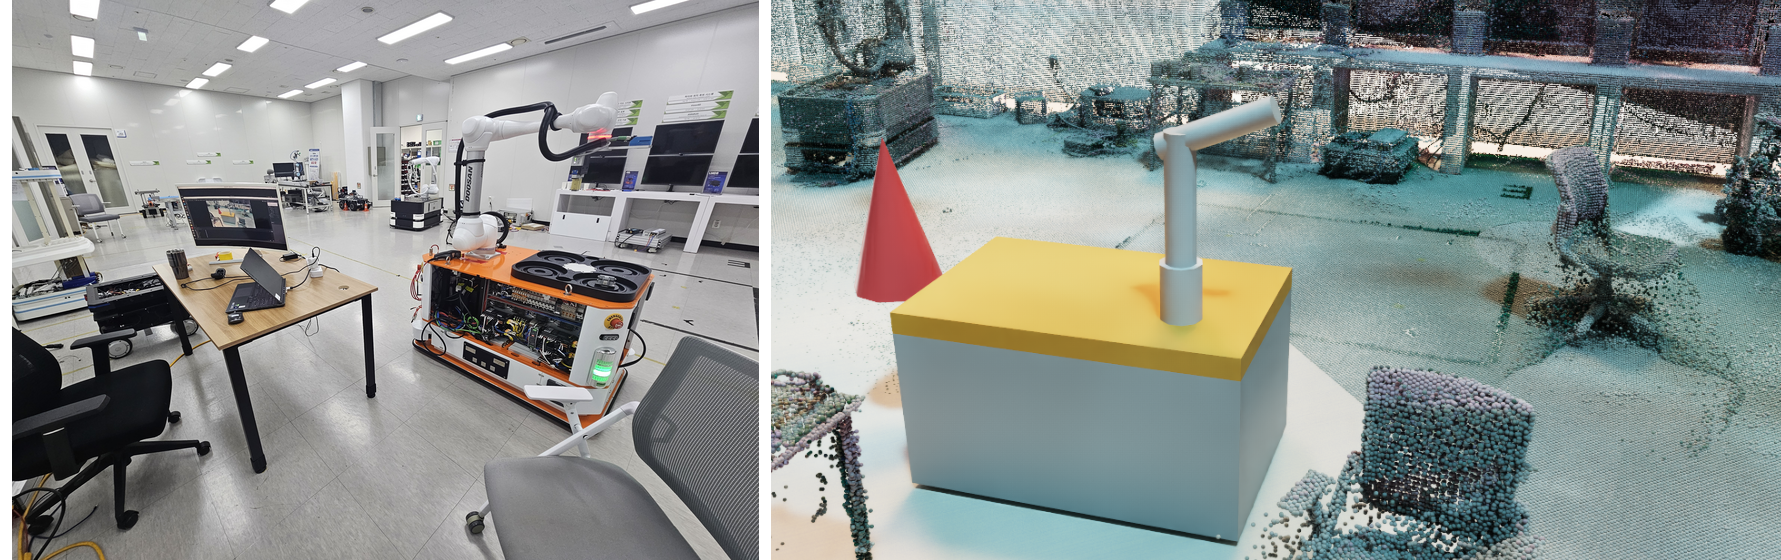
\includegraphics[width=\columnwidth]{fig_pair_room.png}}
\caption{Test facility (left) and its generated twin during the live
session (right). The yellow body with the white column is the AMMR
proxy model; the red cone is the draggable navigation-goal marker.}
\label{figpair}
\end{figure}

\begin{figure}[htbp]
\centerline{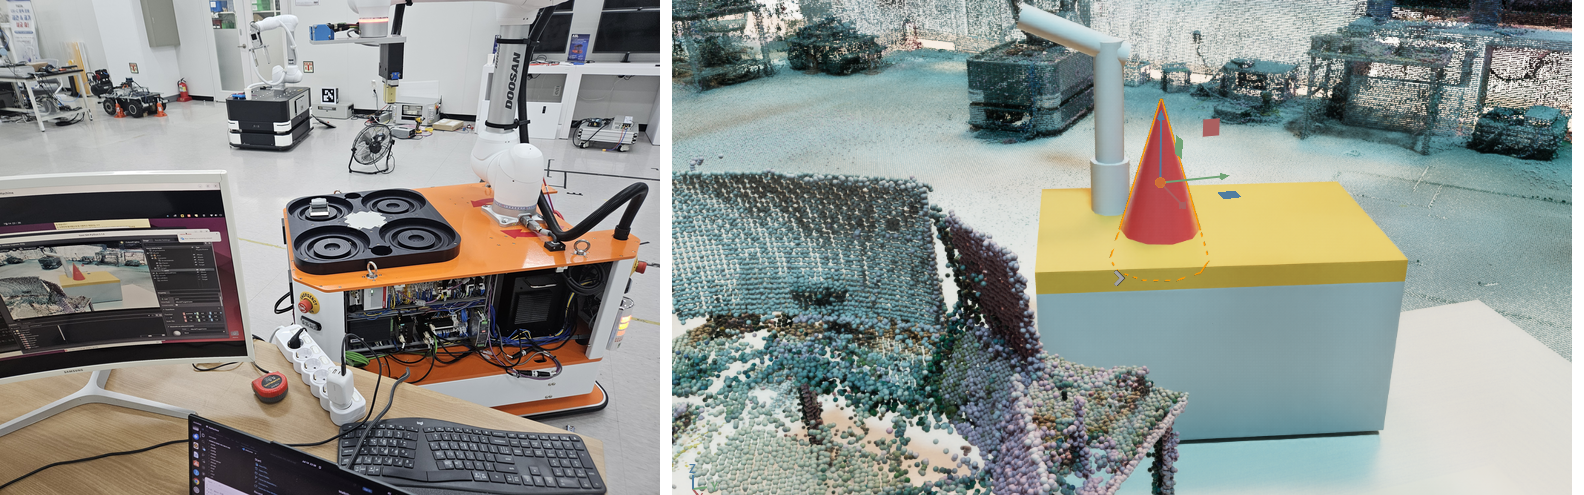
\includegraphics[width=\columnwidth]{fig_pair_goal.png}}
\caption{Simulator-issued navigation goal. Right: twin after arrival,
parked on the goal marker. Left: the physical robot at the
corresponding location.}
\label{figgoal}
\end{figure}

\subsection{Geometric fidelity}
We evaluate metric accuracy at two levels: scene geometry alone, and
the end-to-end twin including localization.

\subsubsection{Scene dimensions} Three room features were
tape-measured and compared against the same dimensions extracted from
the twin's point layer (histogram run-length analysis after wall-axis
alignment). As Table~\ref{tabgeo} shows, all errors are within 2\%,
i.e., the scan-to-simulation conversion itself preserves metric scale
to centimeter level.

\begin{table}[htbp]
\caption{Scene-feature dimensions: tape measure vs. twin point layer}
\begin{center}
\begin{tabular}{|l|r|r|r|}
\hline
\textbf{Feature} & \textbf{Real [m]} & \textbf{Twin [m]} & \textbf{Error} \\
\hline
Window-side wall length & 8.000 & 7.918 & $-1.0$\% \\
Double-door width & 1.700 & 1.680 & $-1.2$\% \\
Workbench row length & 5.010 & 5.100 & $+1.8$\% \\
\hline
\end{tabular}
\label{tabgeo}
\end{center}
\end{table}

\subsubsection{End-to-end positioning} We compare tape-measured
distances between marked floor checkpoints against the corresponding
distances reported by the twin with the robot parked on each
checkpoint. This captures the full error budget---TLS registration,
occupancy quantization, AMCL localization, and anchor
calibration---without requiring a global frame alignment between
ground truth and simulation. Over three checkpoint pairs (0.86, 3.14,
and 1.30 m tape distance) the twin distances deviated by a mean
absolute error of 5.5 cm (RMSE 7.4 cm, max 12.5 cm;
Fig.~\ref{figeval}). The largest deviation occurred on the segment
executed with large in-place rotations and matches the AMCL
repeatability we observed when revisiting the same floor marker
(17 cm), indicating that end-to-end twin accuracy is dominated by the
onboard localization rather than by the reconstructed scene, whose
intrinsic scale error is an order of magnitude smaller
(Table~\ref{tabgeo}).

\begin{figure}[htbp]
\centerline{
\includegraphics[width=\columnwidth]{fig_eval.png}}
\caption{Checkpoint-pair distances, tape measure vs. twin: scatter
against the identity line (left) and signed per-pair error (right).}
\label{figeval}
\end{figure}

\section{Conclusion}
We presented an automated pipeline that turns a terrestrial laser scan
of an indoor industrial space into a physics-enabled Isaac Sim
environment in under 80 seconds, and a live bidirectional digital twin
that couples the generated scene to a real swerve-drive mobile
manipulator over ROS 2. The two-layer scene design (invisible
collision geometry plus dense colored points) yields both metric
navigability and visual fidelity while sustaining near-real-time
simulation of a 3.7 M-point scene. On-site experiments confirmed that
the generated scene preserves metric scale to within 2\% and that
end-to-end twin positioning tracks tape-measured ground truth to
5.5 cm mean absolute error, with simulator-issued goals executed by
the physical robot. Future work includes automatic
semantic decomposition of the scene into articulated objects, mesh
reconstruction for contact-rich manipulation, and multi-robot twins.

% double-blind: Acknowledgment는 camera-ready에서만 추가 (초기 제출본 금지)

\begin{thebibliography}{00}
\bibitem{tao2019} F. Tao, H. Zhang, A. Liu, and A. Y. C. Nee,
``Digital twin in industry: State-of-the-art,'' IEEE Trans. Ind.
Informat., vol. 15, no. 4, pp. 2405--2415, 2019.
\bibitem{blk360} Leica Geosystems, ``BLK360 imaging laser scanner,''
[Online]. Available: https://leica-geosystems.com/products/laser-scanners
\bibitem{isaacsim} NVIDIA, ``Isaac Sim,'' [Online]. Available:
https://developer.nvidia.com/isaac/sim
\bibitem{ransac} M. A. Fischler and R. C. Bolles, ``Random sample
consensus: A paradigm for model fitting with applications to image
analysis and automated cartography,'' Commun. ACM, vol. 24, no. 6,
pp. 381--395, 1981.
\bibitem{ros2} S. Macenski, T. Foote, B. Gerkey, C. Lalancette, and
W. Woodall, ``Robot Operating System 2: Design, architecture, and uses
in the wild,'' Science Robotics, vol. 7, no. 66, 2022.
\bibitem{nav2} S. Macenski, F. Mart\'in, R. White, and J. G. Clavero,
``The Marathon 2: A navigation system,'' in Proc. IEEE/RSJ Int. Conf.
Intell. Robots Syst. (IROS), 2020, pp. 2718--2725.
\bibitem{scan2bim} V. P\u{a}tr\u{a}ucean, I. Armeni, M. Nahangi,
J. Yeung, I. Brilakis, and C. Haas, ``State of research in automatic
as-built modelling,'' Adv. Eng. Informat., vol. 29, no. 2,
pp. 162--171, 2015.
\bibitem{gazebo} N. Koenig and A. Howard, ``Design and use paradigms
for Gazebo, an open-source multi-robot simulator,'' in Proc. IEEE/RSJ
Int. Conf. Intell. Robots Syst. (IROS), 2004, pp. 2149--2154.
\bibitem{orbit} M. Mittal et al., ``Orbit: A unified simulation
framework for interactive robot learning environments,'' IEEE Robot.
Autom. Lett., vol. 8, no. 6, pp. 3740--3747, 2023.
\bibitem{sim2real} W. Zhao, J. P. Queralta, and T. Westerlund,
``Sim-to-real transfer in deep reinforcement learning for robotics: A
survey,'' in Proc. IEEE Symp. Ser. Comput. Intell. (SSCI), 2020,
pp. 737--744.
\bibitem{cyclonedds} Eclipse Foundation, ``Eclipse Cyclone DDS,''
[Online]. Available: https://cyclonedds.io
\end{thebibliography}

\end{document}
